% --------------------------------------
% Chapter 8 Solutions
% --------------------------------------


\subsection{8.1 $\bigstar$}
We can always write $z=re^{i\theta+2\pi i k}$, where $k$ is some integer. Then $f(z)=z^a=r^a e^{i\theta a+2\pi i ka}$. For 0 turns, $k=0$ and $z^a=r^a e^{i\theta a}$. The Riemann sheets will join together when $2\pi i ka=2\pi i p$, where $p$ is some integer.\footnote{The sheets meet up when $f(z)$ after 0 turns is equal to $f(z)$ after $k$ turns.} This implies that $ka=p\implies a=p/k$. Now suppose $a$ is irrational. By definition, there are no integers $p$ and $k$ such that $a=p/k$. Hence the spiralling sheets will not join again for any number of turns.  \\ \\  
If $a$ is rational, i.e. of form, $a=m/n$ (remembering that $m$ and $n$ have no common factors) then $m/n=p/k\implies p=mk/n$. This equation is first satisfied when $k=n$, and so the sheets meet up after $n$ turns.


\subsection{8.4 $\bigstar \bigstar (\bigstar)$}
This problem is a great deal harder than what Penrose has rated it. It is likely that he made a mistake with the phrasing of the question, and instead meant one had to show that the mapping preserves origin-centred circles, which is much easier.\footnote{I have checked the official correction page for Road to Reality, and there is no correction listed. Perhaps there is an easier way than I know of!}  Indeed, such a circle is given $C=Re^{i\theta}$ where $0\leq\theta<2\pi$. Then if $f(z)=z^{-1}$, then $f(C)=R^{-1}e^{-i\theta}$ which is evidently another origin-centred circle of radius $\tilde{R}=R^{-1}$ and of opposite orientation.\\ \\ 
However, we also want to show the general case. We give here two proofs. The first is the most elegant, but the second is perhaps more direct, and is nice and geometrical.

\subsubsection*{Proof 1: Apollonius}
We use an ancient theorem, due to Apollonius, which gives a useful representation of an arbitrary circle. It states:\\ \\ \emph{Let $t$ be some positive real number. Let $a,b$ be arbitrary complex numbers such that $a\neq b$. Then the locus of points satisfying }
$$|z-a|=t|z-b|$$
\emph{is a circle with radius $R$ and centre $C$, where}
$$R=\frac{t|a-b|}{|t^2-1|} \ \ \ \ \ \ \ \ \ \ C=\frac{t^2 b -a}{t^2-1}$$
Now for a circle centred at $C\neq 0$ of radius $R$, we obviously have that $|z-C|=R$. Now if we apply the transformation $f(z)=z^{-1}$, we have that every point $z \to z^{-1}$, so 
\begin{align*}
|z-C|=R\to |z^{-1}-C|=R&\implies \frac{|z|}{|C|}\left|z^{-1}-C\right|=R\cdot \frac{|z|}{|C|}\\
&\implies\left|z-\frac{1}{C}\right|=\frac{R|z|}{|C|}
\end{align*}
But this is exactly the form of the theorem of Apollonius, and so the inversion of the circle is another circle. Now the observant reader will notice two special cases, when $C=0$ and when $|C|=R$. The case $C=0$ is trivial to show the preservation of the circle. Now when $|C|=R$, we have that $t=1$ in the theorem, and then the radius of the resulting circle is infinite, and the origin of the circle is at infinity. As Penrose mentions somewhere, such a circle is just an infinitely long straight line.

\subsubsection*{Proof 2: Geometry}

 We can parametrize an arbitrary circle centred at $k\in\mathbb{C}$, as $C=Re^{i\theta}+k$ with $0\leq \theta<2\pi$. One strategy to show this is to do as we did for the origin-centred case, and show that 
$$\frac{1}{Re^{i\theta}+k}=\tilde{R}e^{i\tilde{\theta}}+\tilde{k}$$
\begin{figure}[h!]
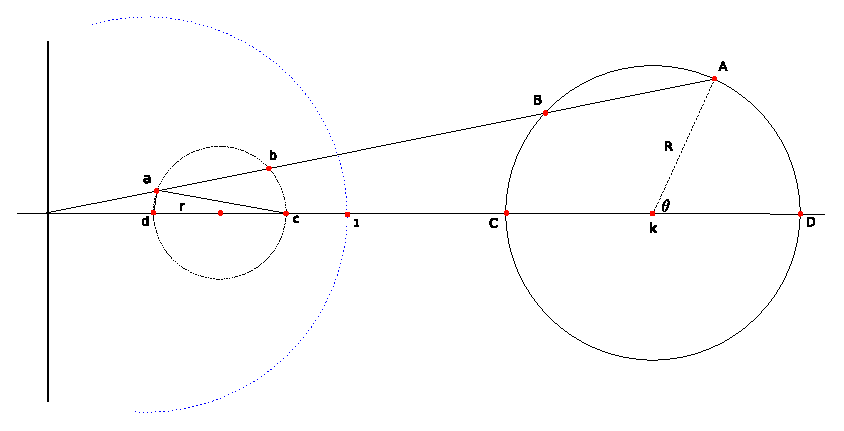
\includegraphics[scale=1.2]{chapters/images/inversion.eps}
\caption{The geometry of the inversion of a circle. }
\end{figure}  

where $\tilde{R}\in\mathbb{R}$, $\tilde{k}\in\mathbb{C}$, and obviously both have no $\tilde{\theta}$ dependance. This can be tried, but quickly one suffocates in the algebra!\footnote{There may an elegant way to do this algebra, but I haven't found it, and not for want of trying!}\\ \\
Lets try a different tactic. We first note that the function $f(z)=z^{-1}=R^{-1}e^{-i\theta}$ can obviously be decomposed into first reflecting all the points about the real-axis, and then inverting the radius. The reflection obviously preserves circles. So lets show that the inversion also does. \\ \\
Consider \textbf{Fig 2}. The big circle is inverted, and we have that $[a]=[A]^{-1}$, $[b]=[B]^{-1}$ etc. Here $[a]$ denotes the magnitude of $[a]$, or distance of $a$ from the origin. The strategy will be to show that the angle $\angle c\hat{a} d=90^{\circ}$. As $A$ is an arbitrary point on the big circle, $a$ will be an arbitrary point on the shape resulting from the inversion of the big circle. But iff for fixed $d$,$c$ every $a$ produces $\angle c\hat{a} d=90^{\circ}$, then we know from circle geometry that $a$ lies on a circle of diameter $[cd]=|[c]-[d]|$.\footnote{The reason for the absoloute magnitude is that we want to keep things general. If the origin was contained within the original circle, then $[c]-[d]$ will be negative.} To show this, we will show that the Pythogarean theorem holds $[ac]^2+[ad]^2=[cd]^2$ for any $a$. But the Pythogarean Theorem only holds iff and only iff $\angle c\hat{a} d=90^{\circ}$.\footnote{The implication $\angle c\hat{a} d=90^{\circ}\implies [ac]^2+[ad]^2=[cd]^2$ is was stated in the beggining of Chapter 2. It is easy to see that the converse $\angle c\hat{a} d=90^{\circ}\implies [ac]^2+[ad]^2=[cd]^2$ must also be true. For suppose $\angle c\hat{a} d=90^\circ$, then $[ac]^2+[ad]^2=[cd]^2$. But suppose I fix the side-lengths $[ac]$ and $[ad]$. Now increasing/decreasing the angle $\angle c\hat{a} d$ will necessarily increase/decrease the hypotenuse $[cd]$. And so any increase/decrease in the angle will break the relation $[ac]^2+[ad]^2=[cd]^2$. So iff the relation holds, the angle must be exactly $90^\circ$.   }   \\ \\
To begin with, suppose we form a triangle between two arbitrary points $a,d$ and the origin $O$. We then have that $[a][A]=1=[d][D]$ from $[A]=a^{-1}$ and $[D]=d^{-1}$.  Then $[a]=([d][A]^{-1})[D]=k [D]$ and $[d]=([a][D]^{-1})[A]=k [A]$ as $k=[d][A]^{-1}=[a][D]^{-1}$. So the triangles $aOd$ and $DOA$ are similar, as the angle $\angle a\hat{O}d=\angle D\hat{O}a$ and the two sides are equal up to a common scale factor. Hence the third side of the two triangles is also related by this scale factor. 
$$[ad]=k[AD]=\frac{[d]}{[A]}[AD]=\frac{[AD]}{[A][D]}$$   
Note that we proved this for arbitrary points, not just the $a$ and $d$ shown in \textbf{Fig 2}. Another simple result we will need (from \textbf{Fig 2}) is that $[AC]^2+[AD]^2=(D-C)^2=4R^2$ as $\angle C\hat{A} D=90^\circ$. \\ \\
We can now state our condition which we wish to show
\begin{align*}
[ad]^2+[ac]^2&=(c-d)^2\\
\implies\ \ \ \ \ \frac{[AD]^2}{[A]^2[D]^2}+\frac{[AC]^2}{[A]^2[C]^2}&=\left(\frac{1}{[D]}-\frac{1}{[C]}\right)^2\\
\implies\ \ \ \ \ [C]^2[AD]^2+[D]^2[AC]^2&=[A]^2\left([D]^2+[C]^2-2[C][D]\right)\\
&=4[A]^2R^2
\end{align*} 
Now we need to show that both sides are equal. We can now use coordinates and just churn out the result.\footnote{Some may be worried that I am only dealing with a very particular circumstance, with the original circle centred on the x-axis. But the inversion does not depend on any angle, it has rotational symmetry. So we can always rotate our coordinates so that this is the case.} It can easily be seen that the following are true:
\begin{align*}
[AD]&=2R\sin(\frac{1}{2}\theta) \\
[AC]&=2R\cos(\frac{1}{2}\theta) \\
[A]^2&=R^2\sin^2\theta+(k+R\cos\theta)^2=R^2+k^2+2kR\cos\theta\\
[C]&=k-R \\
[D]&=k+R
\end{align*}
The right-hand side (RHS) becomes
\begin{align*}
[C]^2[AD]^2+[D]^2[AC]^2&=(k-R)^2[2R\sin(\frac{1}{2}\theta)]^2+(k+R)^2[2R\cos(\frac{1}{2}\theta)]^2\\
&=4k^2R^2+4R^4+8kR^3(\cos^2(\frac{1}{2}\theta)- \sin^2(\frac{1}{2}\theta))\\
&=4R^2(k^2+R^2+2kR \cos\theta)
\end{align*}
where in the last line we made use of the identity $\cos(2\theta)=\cos^2\theta-\sin^2\theta$. Now the left-hand side:
\begin{align*}
4[A]^2R^2&=4\cdot(R^2+k^2+2kR\cos\theta)\cdot R^2\\
&=4R^2(R^2+k^2+2kR\cos\theta)
\end{align*}
which is the same as the RHS. Hence the Pythogorean identity holds, and $\angle c\hat{a} d=90^{\circ}$, and hence the image of the inversion of a circle is another circle. We note also that the argument used was completely general. It did not depend on where the original circle actually was.\footnote{The method used was inspired by the one used by Needham \cite{need}, but with major modifications. He used a beautifully simple argument using the similar triangle property, but one had to consider seperately the case where the origin is contained in the original circle, and a few other considerations were needed to take care of the case where the original circle overlaps the unit circle.}  





